\chapter{Generalized Linear Models \label{chapter:glms}}

Linear and logistic regression, which we have seen already in Chapters~\ref{chapter:classification}, \ref{chapter:regression}, \ref{chapter:linreg}, and \ref{chapter:logreg}, are members of a broader class of supervised learning models called \textbf{generalized linear models (GLMs)}. In GLMs, the outcome variable, $y$, is assumed to follow a probability distribution of a particular type. For example, in linear regression, $y$ follows a normal distribution. In logistic regression, $y$ is binary $\left( y \in \{0, 1\} \right)$ and follows a Bernoulli distribution\footnote{In \textbf{grouped} logistic regression, it follows a binomial distribution.}. The expected value, or mean, of the outcome distribution is related to a \textbf{linear combination} of the predictors, $\beta_0 + \beta_1 x_1 + \dots + \beta_p x_p$, via a model-specific \textbf{link function}.

GLMs, like maximum likelihood (Chapter~\ref{chapter:mlebasics}), are normally considered an advanced topic. However, they provide a nice example of how the same formalism -- modeling the response variable using a probability distribution, assuming a certain form for the predictors, optimizing the whole thing using maximum likelihood -- can be applied to solve different-looking problems. They are also a good entryway into the sorts of optimization tasks performed by graphical models and deep learning algorithms. 

%%%%%%%%%%%%%%%%%%%%%%%%%%%%%%%%%%%%%%%%%%%%%%%%%%%%%%%%%%%%%%%%%%%%%%%%%%%%%%%

\section{Model Assumptions}

GLMs require us to make several assumptions which affect both our choice of model and our interpretation of model output:

\begin{enumerate}
\item We assume that the outcome follows a certain type of distribution (e.g. Bernoulli distribution for a logistic regression model, normal for linear, etc.) conditional on the predictors. This assumption is baked into the model structure. It is, therefore, important to consider whether the outcome distribution you chose actually makes sense for your particular problem. It is generally not advisable to use a linear regression model, for example, when your outcome is a count. 
\item We assume that the predictors are fixed and known, and thus have no error associated with their measurements\footnote{Bayesian versions of these models relax this assumption.}.
\item We assume that the predictors enter the model as a linear combination, $\beta_0 + \beta_1 x_1 + \dots + \beta_p x_p$. This is why GLMs are referred to as ``linear models''. 
\item We assume that the $n$ samples in our dataset are collected independently, so that the errors of the $n$ sample outcomes are uncorrelated\footnote{Think back to our formulation of the likelihood in Chapter~\ref{chapter:mlebasics} and how it depended on the samples' being independent and identically distributed, or iid.}.
\end{enumerate}

%%%%%%%%%%%%%%%%%%%%%%%%%%%%%%%%%%%%%%%%%%%%%%%%%%%%%%%%%%%%%%%%%%%%%%%%%%%%%%%

\section{Notation for the Predictors}

As mentioned above, GLMs assume that the predictors enter the model as a linear combination. A linear combination is an expression constructed from a set of terms by multiplying each term by a constant and adding the results. We denote the number of predictors in the model by $p$ and the vector of predictors by $x$, where
$$ x = \begin{bmatrix}
1 \\
           x_{1} \\
           x_{2} \\
           \vdots \\
           x_{p}
         \end{bmatrix} $$
and we have included a ``1'' as the first element to allow for an \textbf{intercept}. We write $x^{(i)}$ to denote the vector of predictors associated with the $i$th training example. The coefficients of the linear combination (i.e. the model parameters we are hoping to learn) are denoted by:
$$ \beta = \begin{bmatrix}
\beta_0 \\
           \beta_{1} \\
           \beta_{2} \\
           \vdots \\
           \beta_{p}
         \end{bmatrix} $$
and we often express the linear combination as an \textbf{inner product}, or \textbf{dot product}, of the two vectors, written as
$$ \beta^T x = \beta_0 + \sum_{j=1}^p \beta_j x_j. $$
This is just notational shorthand. 
\vspace{3mm}

\begin{question}{}
We saw the details of linear and logistic regression models in Chapters~\ref{chapter:linreg} and \ref{chapter:logreg} and discussed the limitations of predictors' entering as a linear combination. What are some of those limitations?
\end{question}

\begin{question}{}
Just to confirm that you understand this notation, write out the form of $\beta^Tx$ for a model with (a) one predictor, (b) three predictors. Write both the general form and the form for one training example, $x^{(i)}$. 
\end{question}

%%%%%%%%%%%%%%%%%%%%%%%%%%%%%%%%%%%%%%%%%%%%%%%%%%%%%%%%%%%%%%%%%%%%%%%%%%%%%%%

\section{Modeling the Outcome}

Generalized linear models model the expected value of the outcome, $E[y]$, as a function of this linear combination of predictors.

\subsection{Linear Regression}

In linear regression, we assume that the outcome, $y$, follows a normal distribution (see Section~\ref{sect:normal}), whose mean is controlled by the values of the predictors. Recall that the normal distribution is a continuous probability distribution with the following properties:
$$ p(y) = \frac{1}{\sqrt{2 \pi \sigma^2}} e^{-\frac{(y-\mu)^2}{2 \sigma^2}} \qquad  E[y] = \mu \qquad \text{var}(y) = \sigma^2 $$
where $y \in \mathbb{R}$. Its mean, $\mu$, can be any real number. To link $\mu$ to the predictors, therefore, we simply set it equal to $\beta^Tx$, like so:
\begin{equation} E[y] = \mu = \beta^T x \label{eqn:meanlinear} \end{equation}
This is called using the \textbf{identity link}. The relationship between $E[y] = \mu$ and $\beta^T x$ is shown below.

\begin{center}
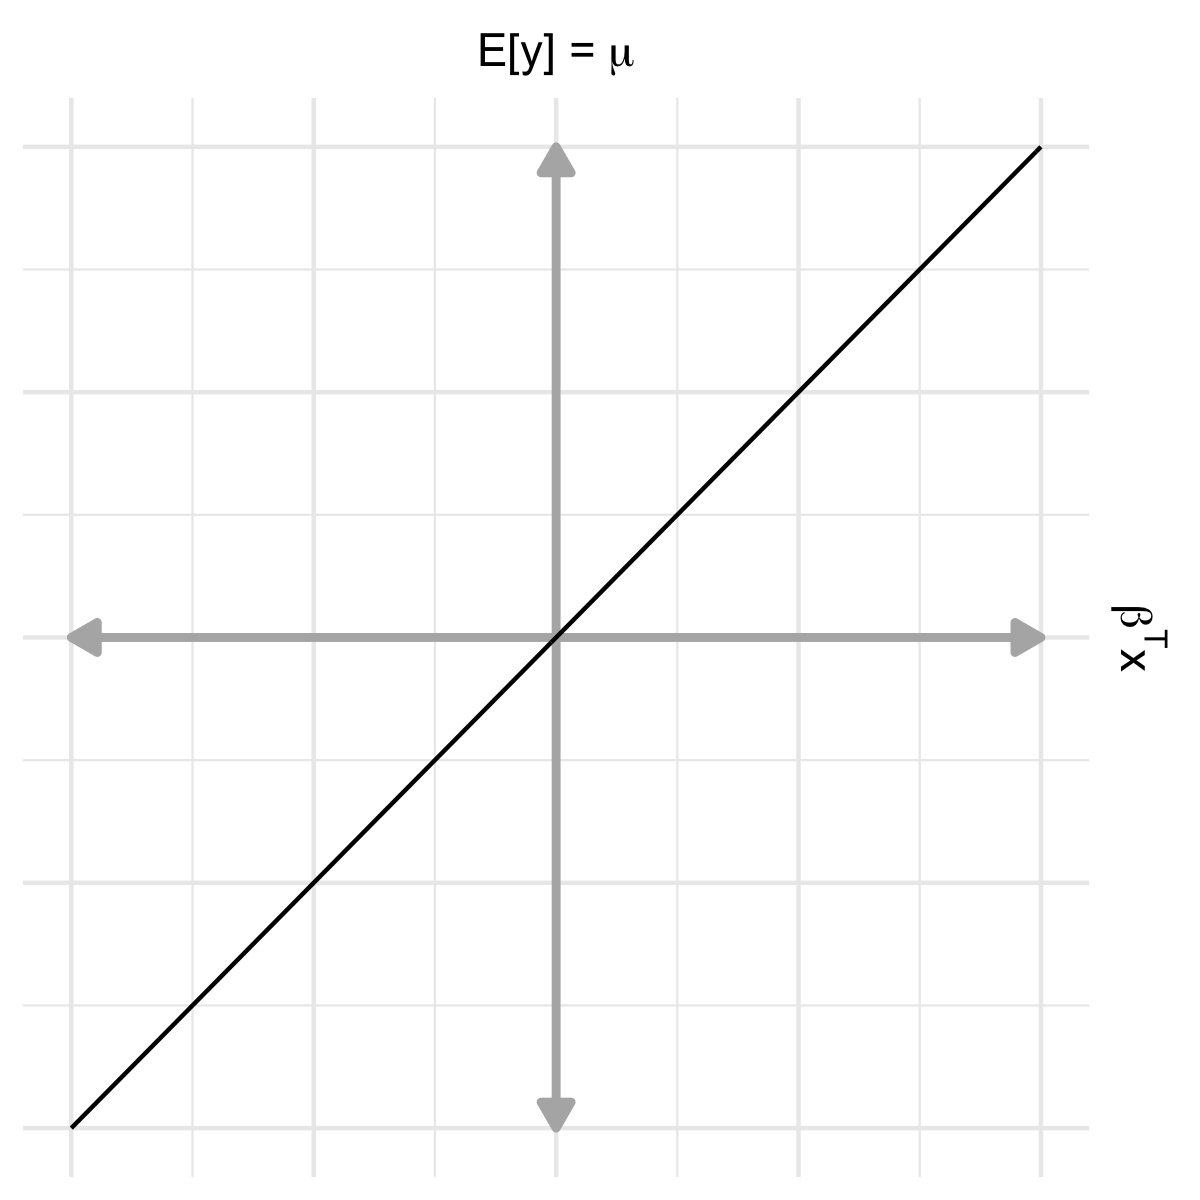
\includegraphics[width=0.5\textwidth]{img/l02-figure1-linreg.png}
\end{center}

\vspace{3mm}

\begin{question}{}
In this model, how much does the mean of the outcome distribution, $\mu$, change as you vary each predictor? For example, if you have $p=3$ predictors, by how much does $\mu$ change as the value of $x_2$ changes by one unit (for example, from $1$ to $2$)? How much does $\mu$ change as the value of $x_2$ changes from $3$ to $4$? What about $x_1$ and $x_3$?
\end{question}

\subsection{Logistic Regression}

In logistic regression the outcome, $y$, is either $0$ or $1$. We model it using the Bernoulli distribution (see Section~\ref{sect:bernoulli}), which is a discrete probability distribution with the following properties:
$$ p(y) = \mu^y (1 - \mu) ^ {1-y} \qquad E[y] = \mu \qquad \text{var}(y) = \mu (1 - \mu) $$
where $y \in \{0, 1\}$. Because $\mu$ is a probability, it must be a real number between 0 and 1. No matter how large or small $\beta^T x$ gets, the value of $E[y] = \mu$ cannot be outside this range. We therefore apply the \textbf{logistic function}, $f(x) = 1/(1 + \exp(-x))$, which has the range $(0, 1)$, to $\beta^T x$ to squash it:
\begin{equation} E[y] = \mu = \frac{1}{1 + \exp{(-\beta^Tx)}} \label{eqn:meanlogistic} \end{equation}
The relationship between $E[y]$ and $\beta^T x$ is shown below. We typically invert the model to write
$$ \log{\frac{\mu}{1-\mu}} = \beta^T x. $$
The function $\log \left( \mu/(1-\mu) \right)$ is called the logit, and we say we use the \textbf{logit link}.

\begin{center}
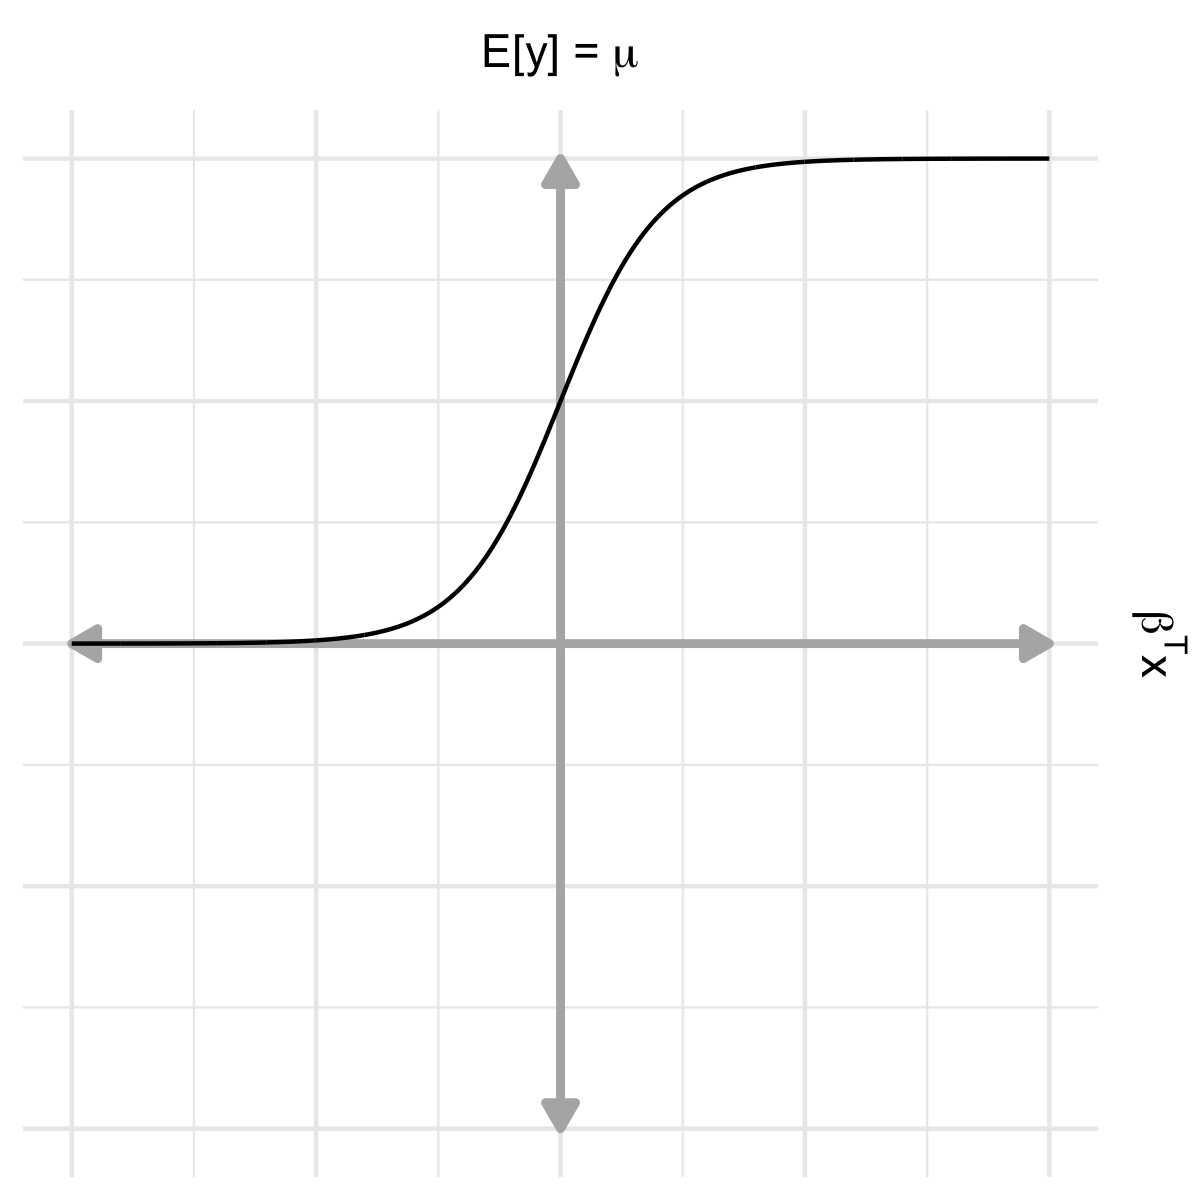
\includegraphics[width=0.5\textwidth]{img/l02-figure2-logistic.png}
\end{center}

\vspace{3mm}

\begin{question}{}
Let's revisit Question~\ref{question:logreglink}. Now that we've described logistic regression in the framework of GLMs, what more can you say about why the model is not of the form
$$ \mu = \beta_0 + \beta_1 x_1 + \dots + \beta_p x_p \text{?}$$
\end{question}

\subsection{Poisson Regression}

In Poisson regression, the outcome is a count. We model the outcome using a Poisson distribution, which is a discrete probability distribution with the following properties (Section~\ref{sect:poisson}):
$$ p(y) = \frac{e^{-\lambda} \lambda^y}{y!} \qquad E[y] = \lambda \qquad \text{var}(y) = \lambda $$
where $y \in 0, 1, 2, \dots$. Because $\lambda$, the mean of the outcome distribution, is the expected value of a count, it must be a real number greater than or equal to zero. In particular, no matter how small $\beta^T x$ gets, the value of $E[y] = \lambda$ cannot be negative. We therefore exponentiate $\beta^T x$ to ensure that $\lambda$ is greater than zero:
\begin{equation} E[y] = \lambda = \exp(\beta^T x) \label{eqn:meanpoisson} \end{equation}
The relationship between $E[y]$ and $\beta^T x$ is shown below. We typically invert the model to write
$$ \log(\lambda) = \beta^T x $$
which is the standard form of the Poisson regression model. We say these models use the \textbf{log link}.

\vspace{3mm}

\begin{question}{}
There are many other generalized linear models. In each case, the mean (expected value) of a probability distribution is related, via a link function, to a linear combination of the predictors. 

Knowing this, how would you create a GLM where the outcome follows an exponential distribution (Section~\ref{sect:exponential})? Which link would you use?
\end{question}

\begin{center}
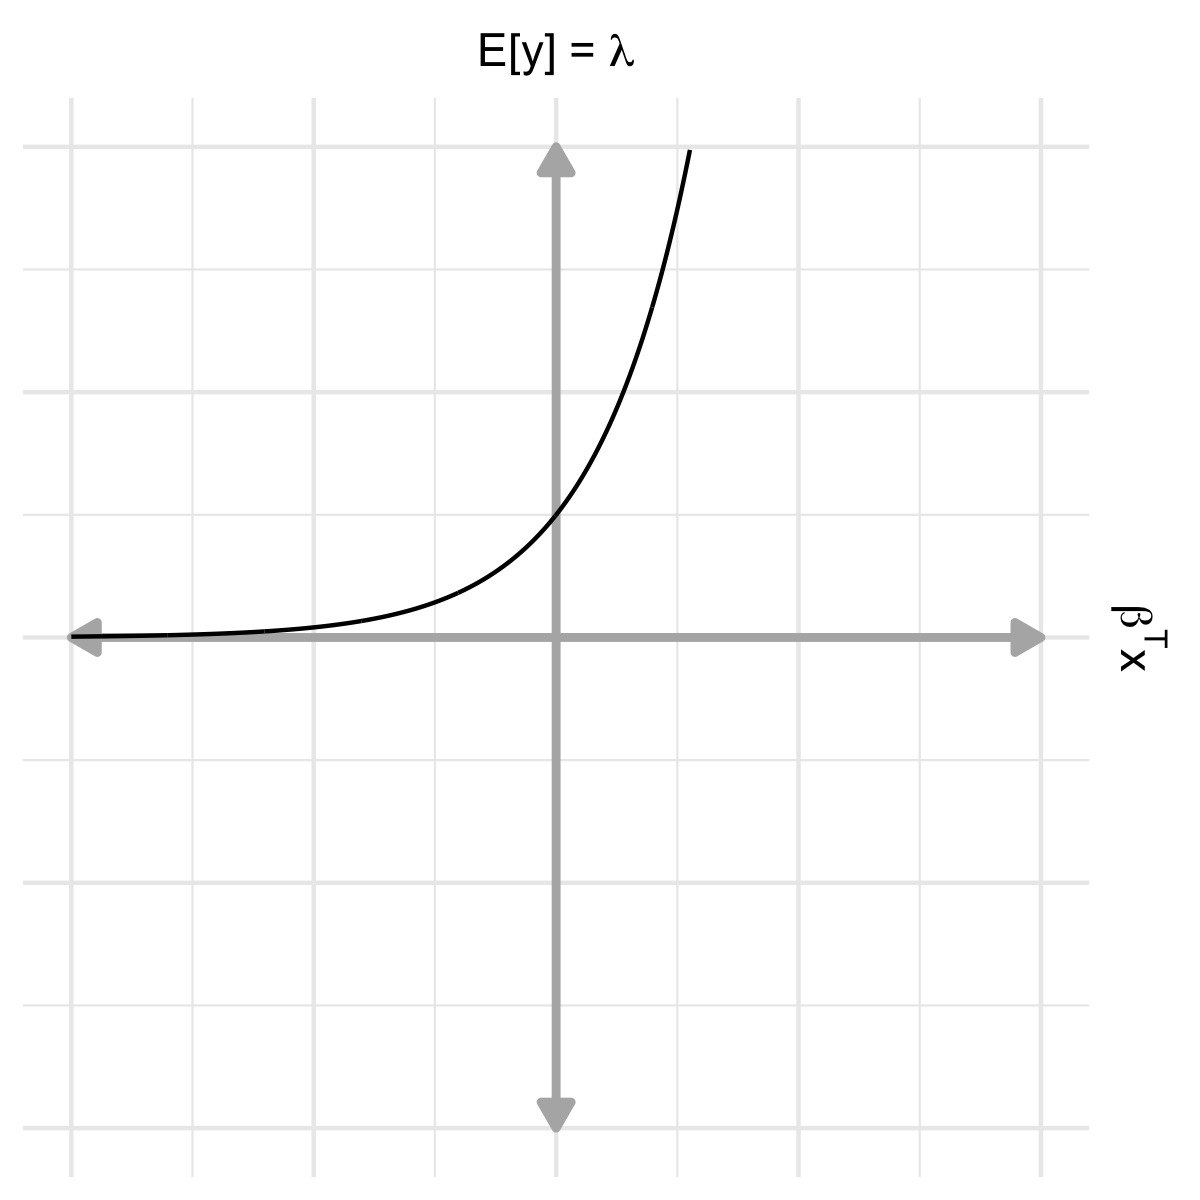
\includegraphics[width=0.5\textwidth]{img/l02-figure3-poisson.png}
\end{center}

%%%%%%%%%%%%%%%%%%%%%%%%%%%%%%%%%%%%%%%%%%%%%%%%%%%%%%%%%%%%%%%%%%%%%%%%%%%%%%%

\section{Maximum Likelihood for GLMs \label{section:mleglms}}

GLMs are fit using maximum likelihood estimation (see Chapter~\ref{chapter:mlebasics}). A full treatment of MLE for GLMs is outside the scope of these notes, but I've put the start of the calculations for each type of model below. The only difference between these calculations and those in Chapter~\ref{chapter:mlebasics} is that now our parameters of interest, the means of our outcome distributions, are functions of our predictors $x_1, \dots, x_p$. Our job is to find the coefficients on those predictors, $\beta_0, \dots, \beta_p$, that provide the best fit between our model and our training data.

\subsection{Linear Regression} 

The likelihood for the linear regression model is:
$$ \mathcal{L}(\mu^{(1)}, \dots, \mu^{(n)}, \sigma) = \prod_{i=1}^n \frac{1}{\sqrt{2 \pi \sigma^2}} \exp \left[ - \frac{(y^{(i)} - \mu^{(i)})^2}{2 \sigma^2} \right] $$
where we use $\mu^{(i)}$ to represent the model's estimate of the mean of the outcome at the position of training example $i$. We can use Equation~\ref{eqn:meanlinear} to rewrite this as a function of the predictors:
$$ \mathcal{L}(\beta, \sigma) = \prod_{i=1}^n \frac{1}{\sqrt{2 \pi \sigma^2}} \exp \left[ - \frac{(y^{(i)} - \beta^T x^{(i)})^2}{2 \sigma^2} \right] $$
Taking the log, we obtain the log-likelihood:
$$ \log \mathcal{L}(\beta, \sigma) = -\frac{n}{2} \log (2 \pi) - \frac{n}{2} \log(\sigma^2) - \frac{1}{2 \sigma^2} \sum_{i=1}^n \left( y^{(i)} - \beta^T x^{(i)} \right)^2 $$
Taking derivatives of the log-likelihood with respect to the $\beta$s, we find that we can maximize the likelihood by minimizing the sum-squares: $\sum_{i=1}^n \left( y^{(i)} - \beta^T x^{(i)} \right)^2$.

\vspace{3mm}

\begin{question}{}
Take a minute to stare at this result. When most people learn linear regression, they learn that these models are fitted by minimizing the sum of squared residuals (see Chapter~\ref{chapter:linreg}). Indeed, linear regression models predate GLMs and are typically fit using ordinary least squares, not maximum likelihood. If you fit a linear regression model in R using the \texttt{lm} package, you're using OLS. If you use the \texttt{glm} package with the argument \texttt{family = "gaussian"}, you're using maximum likelihood. However, both methods will produce the same fitted models. Do you see why this is?
\end{question}

\subsection{Logistic Regression}

The likelihood for the logistic regression model is:
$$ \mathcal{L}(\mu^{(1)}, \dots, \mu^{(n)}) = \prod_{i=1}^n {\mu^{(i)}}^{y^{(i)}} (1-\mu^{(i)})^{1 - y^{(i)}} $$
Rewriting this as a function of the predictors, we get:
$$ \mathcal{L}(\beta) = \prod_{i=1}^n \left( \frac{1}{1 + \exp(-\beta^T x^{(i)})} \right)^{y^{(i)}} \left( \frac{\exp(-\beta^T x^{(i)})}{1 + \exp(-\beta^T x^{(i)})} \right)^{1 - y^{(i)}} $$
Taking the log, we obtain the log-likelihood:
$$ \log \mathcal{L}(\beta) = \sum_{i=1}^n \left[ y^{(i)} \beta^T x^{(i)} - \log \left(1 + \exp(\beta^T x^{(i)}) \right) \right] $$
Again, we will take derivatives of the log-likelihood with respect to the $\beta$s to maximize it. However, we cannot solve for the optimal $\beta$s analytically in this case. Numerical optimization methods are used to find the maximum likelihood estimates, $\hat{\beta}_0, \hat{\beta}_1,$ etc.

\subsection{Loglinear (Poisson) Regression}

The likelihood for the Poisson regression model is:
$$ \mathcal{L}(\lambda^{(1)}, \dots, \lambda^{(n)}) = \prod_{i=1}^n \frac{{\lambda^{(i)}}^{y^{(i)}} e^{-\lambda^{(i)}}}{y^{(i)}!} $$
Rewriting this as a function of the predictors, we get:
$$ \mathcal{L}(\beta) = \prod_{i=1}^n \frac{\exp{(y^{(i)} \beta^T x^{(i)})} e^{-\exp{(\beta^T x^{(i)})}}}{y^{(i)}!} $$
Taking the log, we obtain the log-likelihood:
$$ \log \mathcal{L}(\beta) = \sum_{i=1}^n \left[ y^{(i)} \beta^T x^{(i)} - \exp(\beta^T x^{(i)}) - \log (y^{(i)}!) \right] $$
As with logistic regression, we cannot solve for the optimal $\beta$s analytically; numerical optimization methods are used. 
\vspace{1mm}

\begin{question}{}
Think of the log-likelihood as measuring the height of a hill. Your data, 
$$\left\{x^{(1)},\dots,x^{(n)}\right\}$$ 
don't change, so we don't care about their effect on the height. What we care about are the parameters, $\beta_0, \dots, \beta_p$. For each combination of those $p+1$ parameters, the height changes. We want to find the combination of parameters that puts us at the top of the hill. 

The first derivative of the log-likelihood with respect to one of the parameters, $\beta_j$, is
$$ \frac{\partial \log \mathcal{L}}{\partial \beta_j} $$
and the vector of all of these first derivatives for $\beta_0, \dots, \beta_j$ is called the \textbf{gradient}. Evaluated at a particular set of parameters, the gradient tells you how steep your hill is in the direction of each of your $p+1$ parameters. How could you use this information to maximize the likelihood? You don't need to do any math. Just say how you would do it.
\end{question}

\begin{question}{}
There are many different numerical optimization algorithms that one can use to maximize the likelihood (i.e., find the top of the hill). One of them is called \textbf{Fisher scoring}. Examine the output of the logistic regression models in Chapter~\ref{chapter:logreg} and the Poisson regression model shown below in Section~\ref{sect:poisreg}. Where do you see the term ``Fisher scoring''? What do you think the term ``Fisher scoring iterations'' refers to?
\end{question}

%%%%%%%%%%%%%%%%%%%%%%%%%%%%%%%%%%%%%%%%%%%%%%%%%%%%%%%%%%%%%%%%%%%%%%%%%%%%%%%

\section{Standard Errors and Hypothesis Tests \label{section:sehyp}}

Here, once again, is the summary output from a logistic regression model of the ER readmissions example from Chapter~\ref{chapter:classification}, reprinted again in Section~\ref{sect:eragain}:
\begin{center}
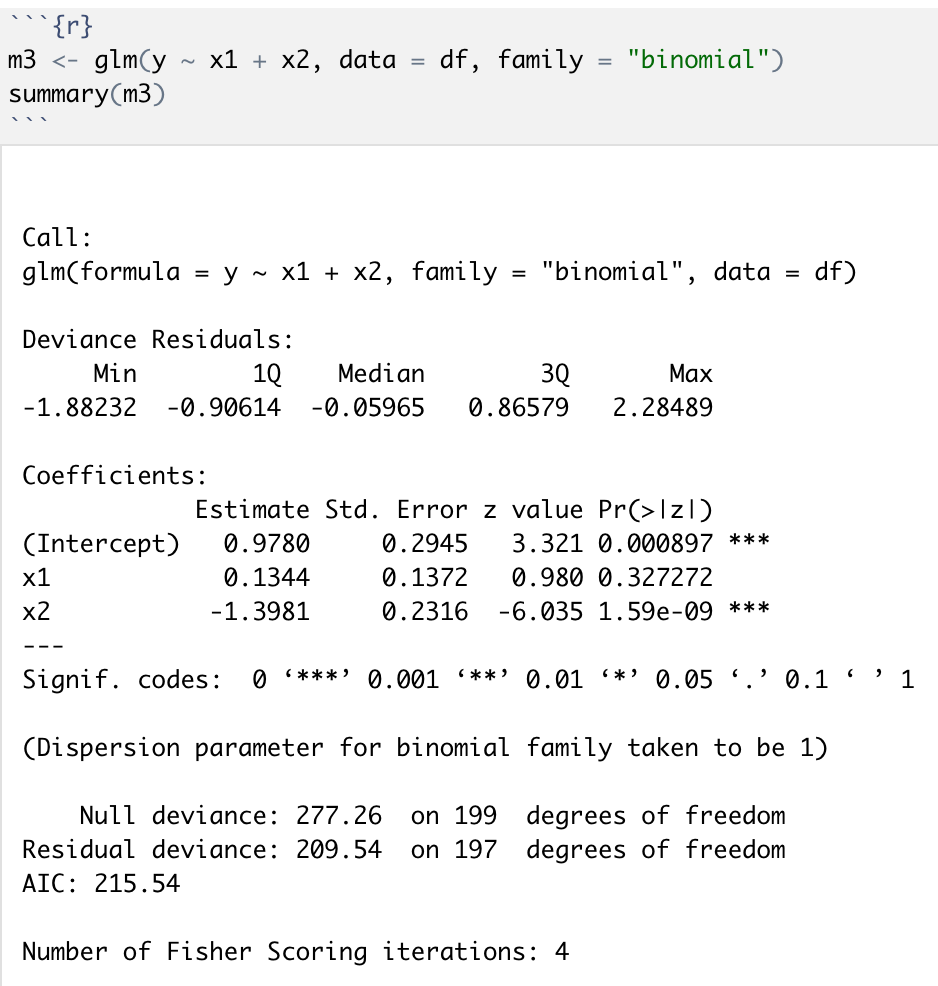
\includegraphics[width=0.7\textwidth]{img/glm-binomial-example.png}
\end{center}
As we discussed in Chapter~\ref{chapter:logreg}, the magnitudes of the coefficients in these models matter, but they are only important in relation to:
\begin{enumerate}
\item The scale on which the predictors are measured. 
\item The amount of uncertainty the model has about their values.
\end{enumerate}
For example, if a predictor varies only across a tiny range of values, its model coefficient may be large, since it quantifies the change in the link-function-transformed outcome when the predictor changes by 1.0. However, that doesn't mean that the predictor itself is important to the outcome\footnote{This is one reason many advocate \textbf{scaling} and \textbf{centering} predictors before fitting a model. Centering means subtracting the mean value of a predictor from all of its individual measurements so that the mean of each centered predictor is zero. Scaling means dividing the values of each predictor by their standard deviation, so that the standard deviation of each predictor is 1.0. This enables the relative magnitudes of the model coefficients to be compared directly.}.

Similarly, the model may be highly uncertain about a coefficient's value, owing to factors like a small dataset (small $n$) or collinearity (correlations) among the predictors. Mathematically, high uncertainty means that the value of the likelihood doesn't change very rapidly as you move away from the maximum likelihood estimate of a coefficient. For example, here is how the log-likelihood for the logistic regression example above changes when we vary $\beta_1$ (the coefficient of $x_1$), keeping $\beta_0$ (the intercept) and $\beta_2$ (the coefficient of $x_2$) fixed at their MLEs: 
\begin{center}
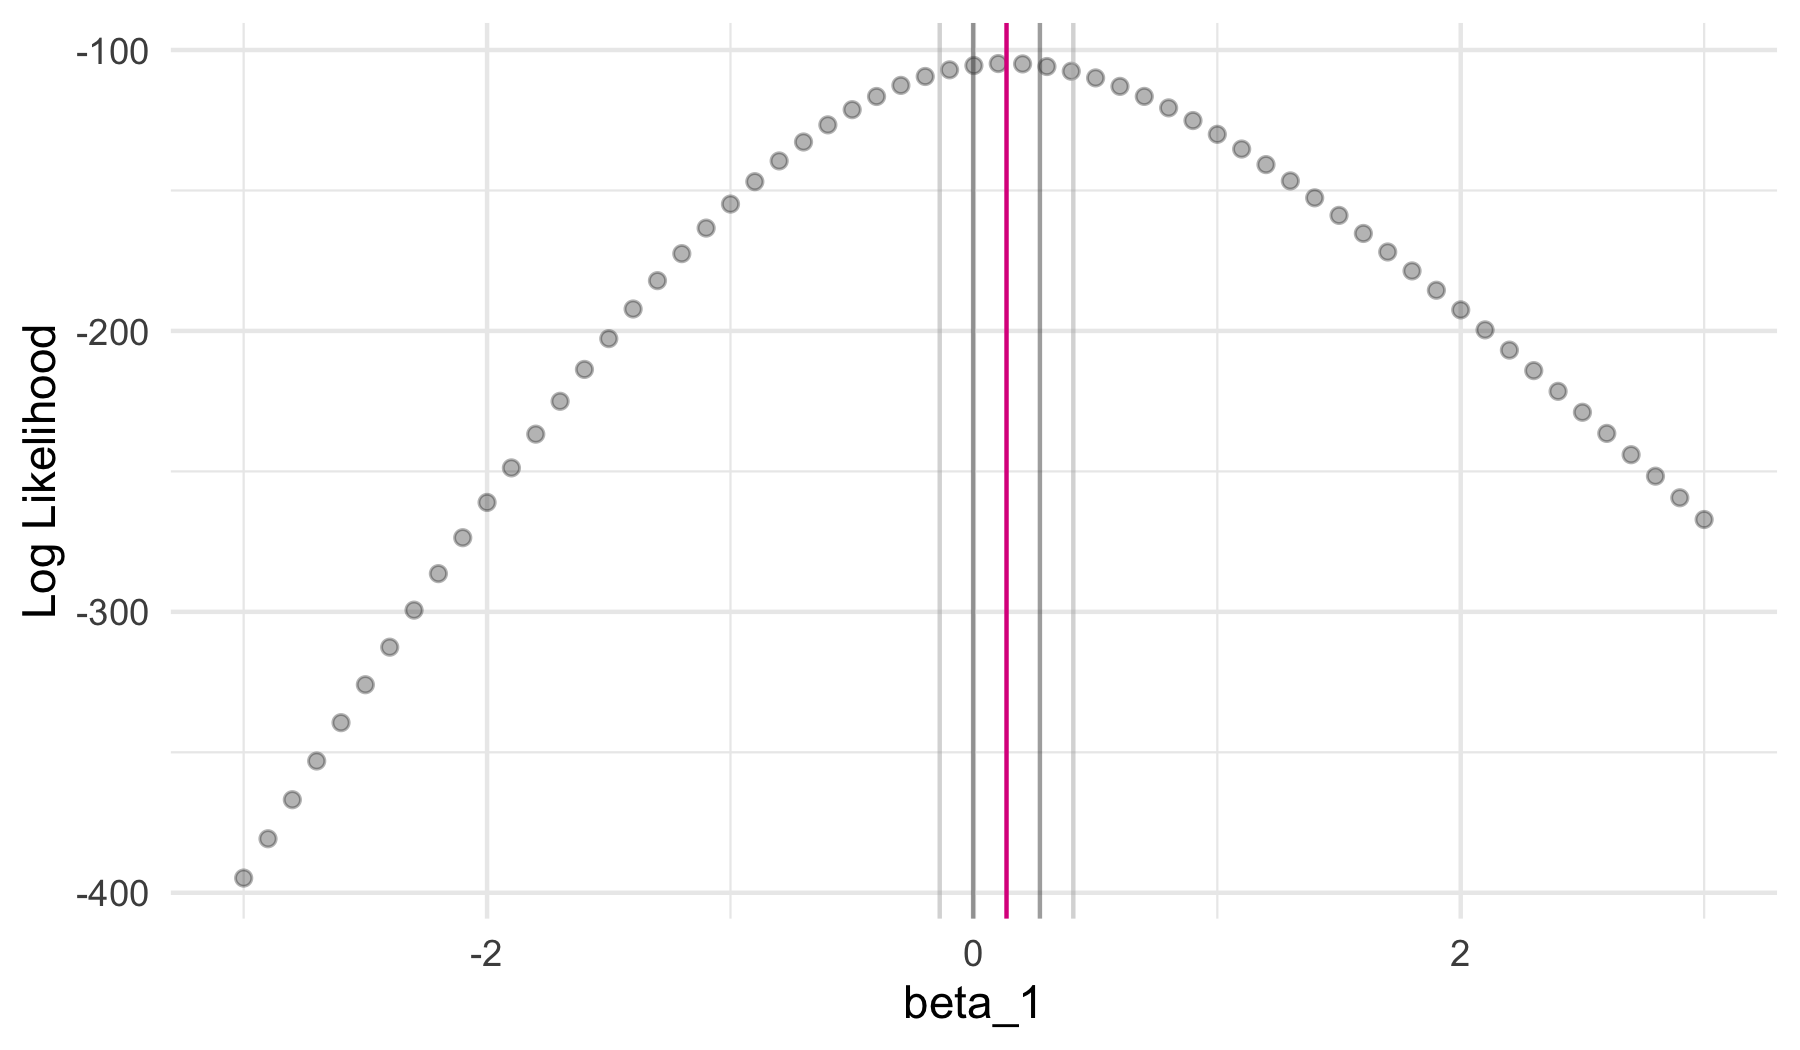
\includegraphics[width=0.7\textwidth]{img/esl-logistic-beta1.png}
\end{center}
The gray vertical lines are related to the \textbf{standard error} of the model coefficient, which is in turn related to the ``flatness'' of the likelihood surface around the MLE. The gray lines are situated at 1 and 2 standard errors away from the MLE in either direction. You can see that in the case of $\beta_1$, the gray lines overlap zero. The value zero (no effect) is a plausible estimate of the impact of $x_1$ on the outcome. 

Contrast this with how the log-likelihood varies around the MLE for $\beta_2$:
\begin{center}
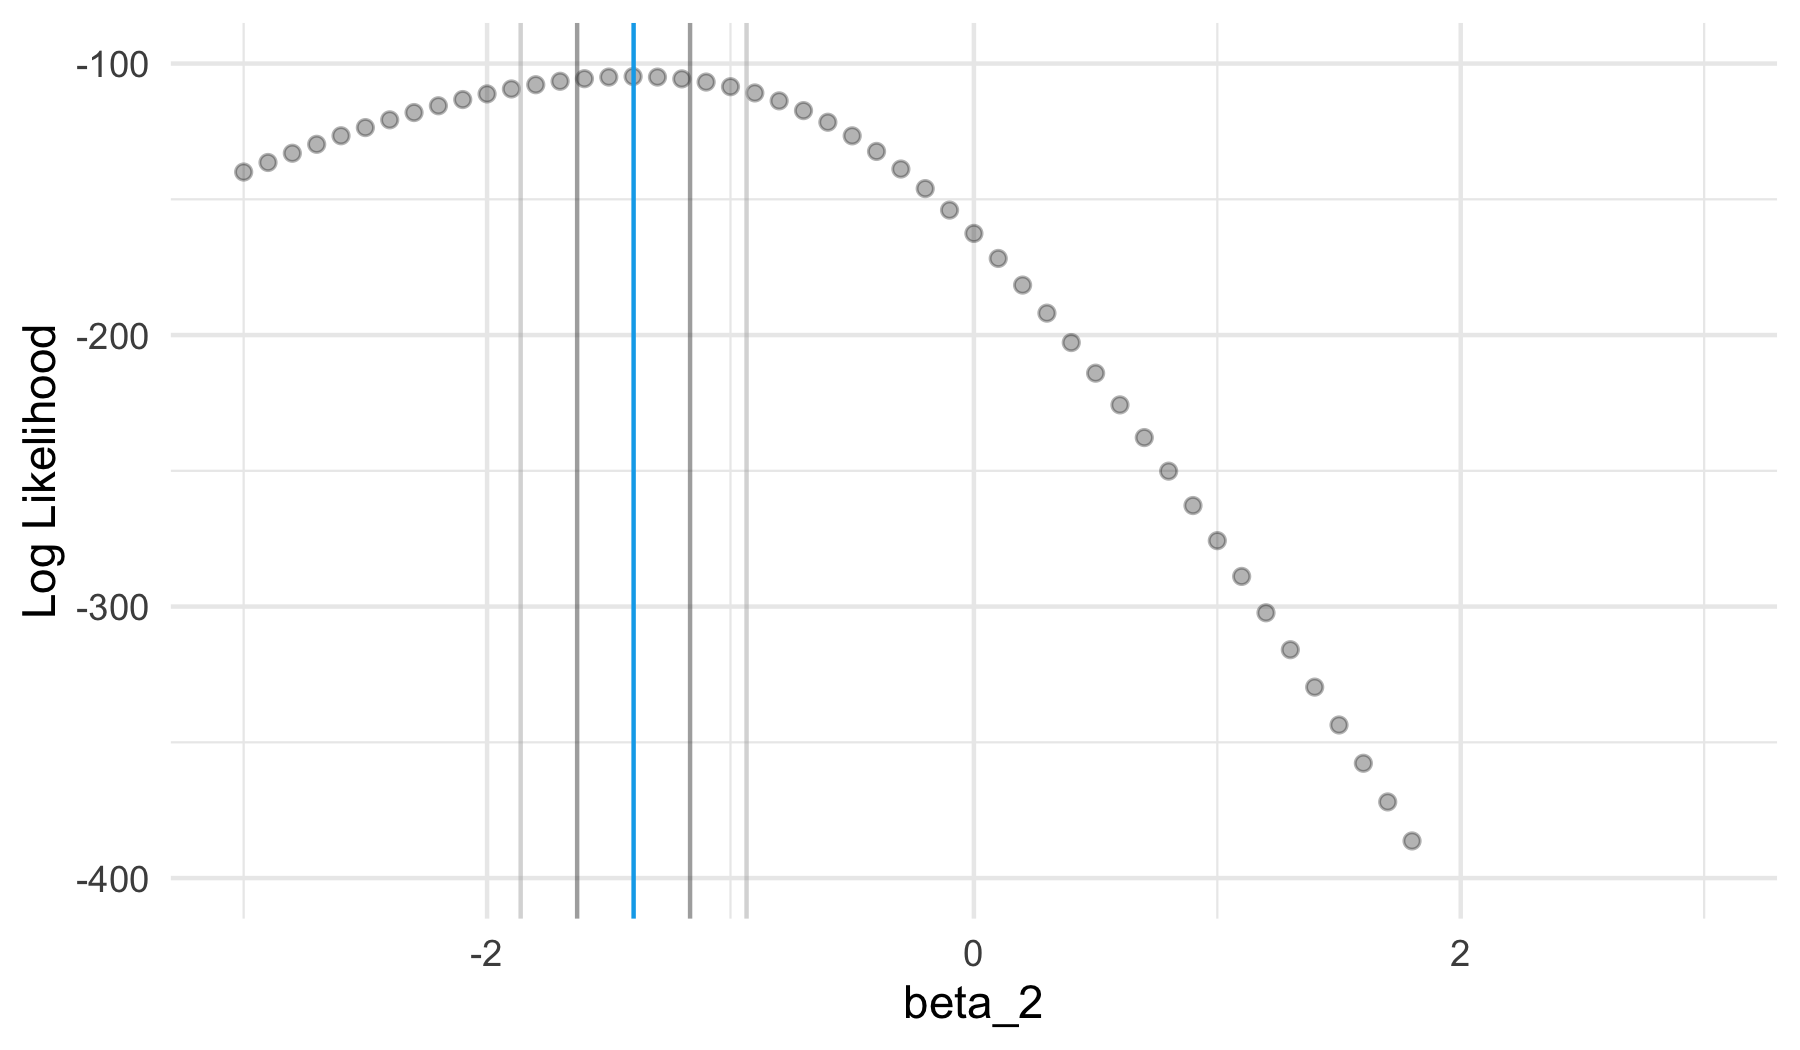
\includegraphics[width=0.7\textwidth]{img/esl-logistic-beta2.png}
\end{center}
Here the standard error is larger, but the magnitude of the coefficient is also larger, so the range of the gray lines does not overlap zero.

\begin{question}{}
These findings are reflected in the relative values of the Z-statistic (\texttt{z value}) and P-value (\verb|Pr(>|z|)|) in the model output for the two coefficients. With that in mind, let's reconsider Question~\ref{question:nulllogregexample}. How do these likelihood plots and the null distributions shown in Question~\ref{question:nulllogregexample} convey the same information?
\end{question} 

%%%%%%%%%%%%%%%%%%%%%%%%%%%%%%%%%%%%%%%%%%%%%%%%%%%%%%%%%%%%%%%%%%%%%%%%%%%%%%%

\section{Example: Nesting Horseshoe Crabs Dataset \label{sect:poisreg}}

Let's examine some output from a Poisson regression model, which is a type of GLM with which you may not already be familiar. 

These data come from a study of nesting horseshoe crabs. Each of the 173 observed female horseshoe crabs had a male crab resident in her nest. The study investigated factors affecting whether the female crab had any other males, called \emph{satellites}, residing nearby. (Source: Agresti, \emph{Categorical Data Analysis}, Table 4.3. Data courtesy of Jane Brockmann, Zoology Department, University of Florida; study described in \emph{Ethology} \textbf{102}: 1-21, 1996.)

\begin{center}
\texttt{\small
\begin{tabular}{ll}
\toprule
SATELL & Number of satellites \\
COLOR & Color of the female crab \\
& (1 = light medium, 2 = medium, 3 = dark medium, \\
& 4 = dark) \\
SPINE & Spine condition \\
& (1 = both good, 2 = one work or broken, \\
& 3 = both worn or broken) \\
WIDTH & Carapace width of the female crab (cm) \\
WEIGHT & Weight of the female crab (g) \\
\bottomrule
\end{tabular}
}
\end{center}

\noindent The GLM output of this model is:

\begin{center}
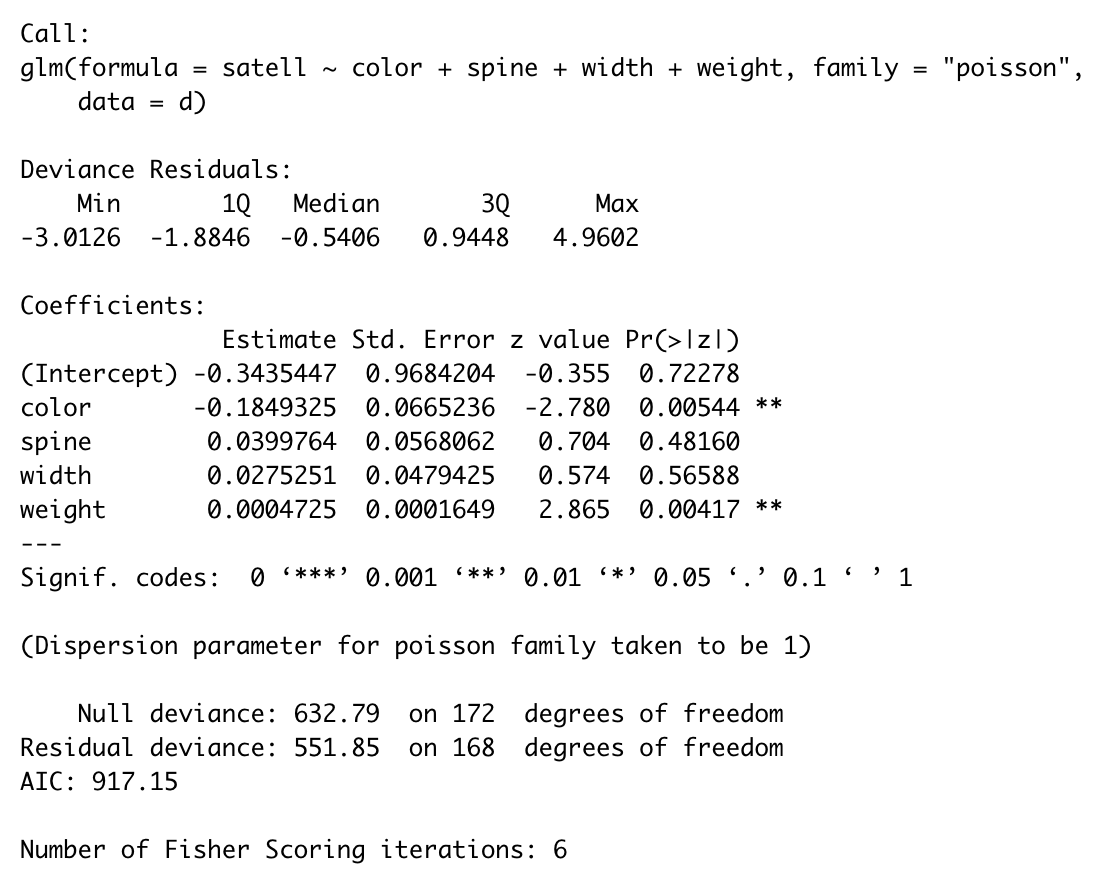
\includegraphics[width=0.8\textwidth]{img/poisson-horseshoe-model.png}
\end{center}

\begin{question}{}
Comment on how the variables \texttt{color} and \texttt{spine} are coded here. Does this make sense in light of what those variables mean?
\end{question}

\begin{question}{}
Interpret the values of each of these coefficients. Based on the coefficient values and their standard errors, which predictor(s) do you think have the greatest impact on the number of male satellites around a nesting female horseshoe crab? 
\end{question}

\begin{question}{}
How could you use a decision tree to model the horseshoe crabs data? What are its advantages and disadvantages relative to Poisson regression (a type of GLM)?
\end{question}

